% !TEX TS-program = xelatex
% !TEX encoding = UTF-8 Unicode
% !Mode:: "TeX:UTF-8"
\documentclass[14pt]{resume}
\usepackage{graphicx}
\usepackage{tabu}
\usepackage{multirow}
\usepackage{multicol}
\usepackage{progressbar}
\usepackage{zh_CN-Adobefonts_external}
\usepackage{linespacing_fix}
\usepackage{cite}

\begin{document}
\pagenumbering{gobble}
% \name{周伟林}
% \basicInfo{
%   \homepage[zhouweilin.cn]{https://zhouweilin.cn/}\
%   \github[github.com/Si3ver]{https://github.com/Si3ver} 
% }
% \basicInfo{
%   \email{izhouwl@163.com}\ 
%   \phone{176-0053-5912}
% }
% \begin{multicols}{2}
%     \Large{
%         \begin{tabu}{ l l }
%             \multirow{5}{1.15in}{
%                 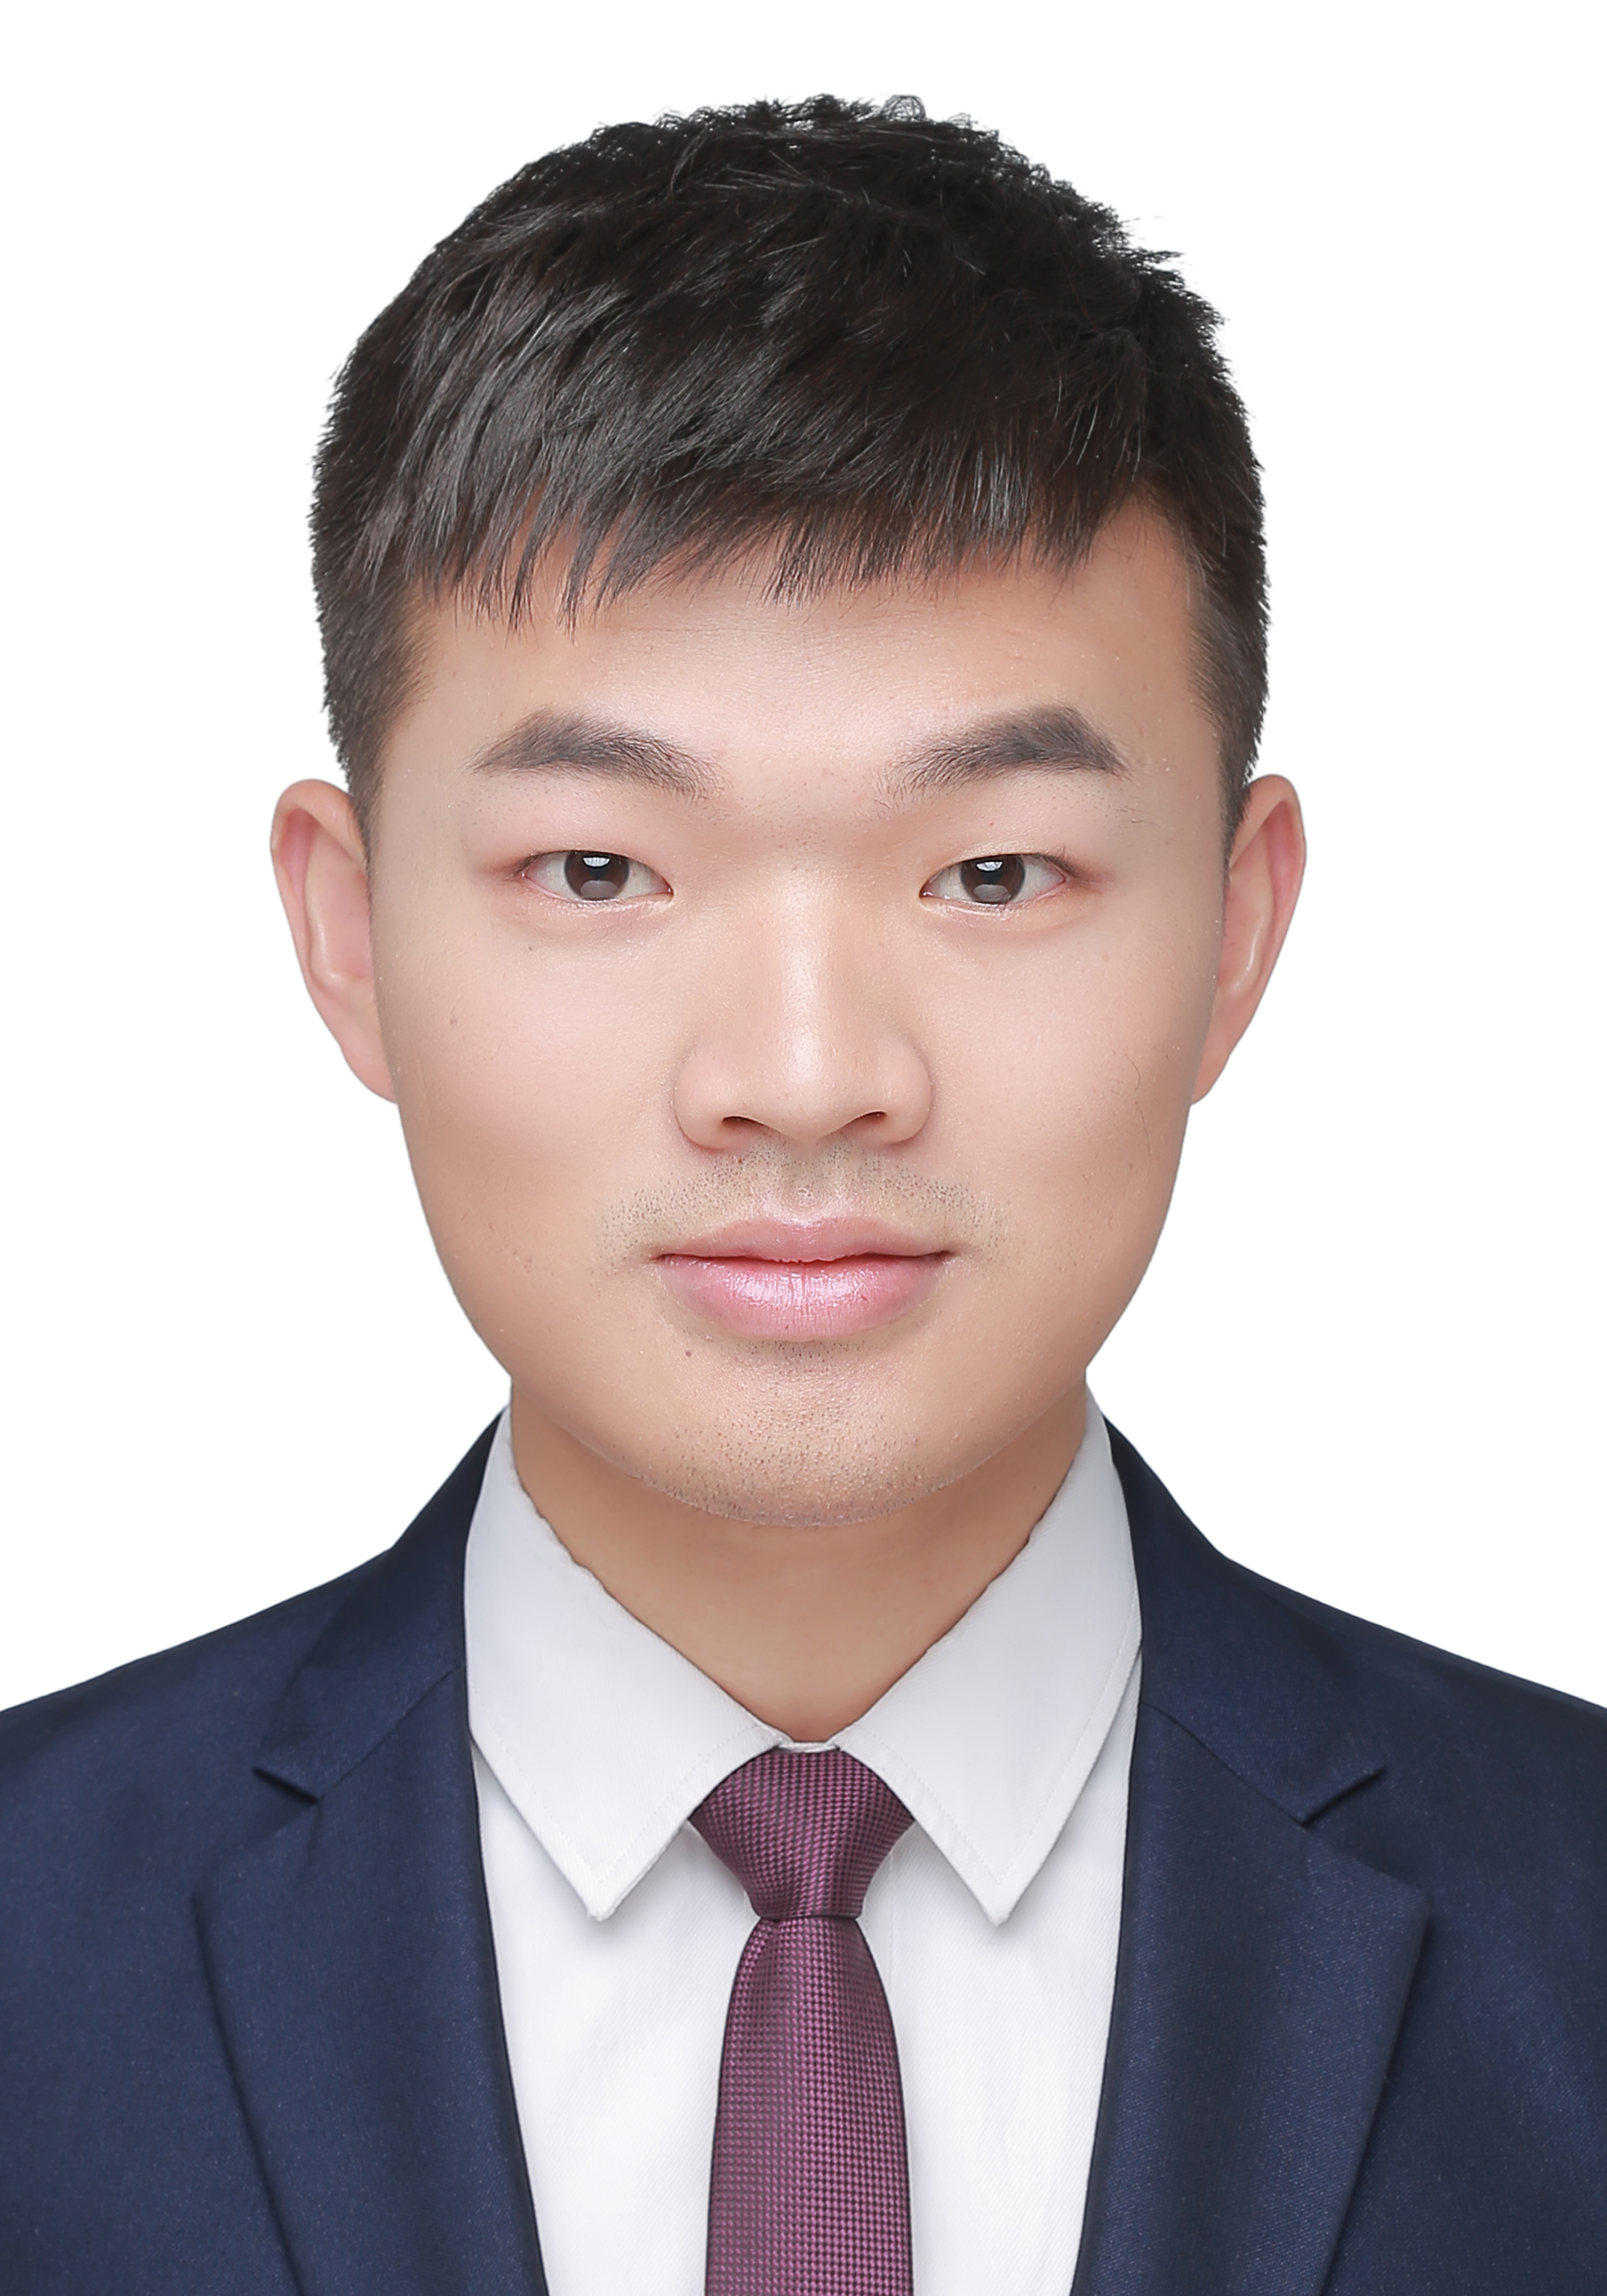
\includegraphics[width=0.88in]{avatar}
%             }
%             & \faBirthdayCake{1995.09.12} \\
%             & \phone{(+86)17600535912} \\
%             & \email{izhouwl@163.com} \\
%             & \homepage[www.zhouweilin.cn]{https://zhouweilin.cn} \\
%             & \github[github.com/Si3ver]{https://github.com/Si3ver} 
%         \end{tabu}
%     }
%     \columnbreak
%     \Large{
%         \begin{tabu}{ l l }
%             \multirow{5}{2.15in}{
%                 \name{周伟林}
%                 \basicInfo{
%                     \faSmileO{意向职位:web前端研发}
%                 }
%             }
%         \end{tabu}
%     }
% \end{multicols}

\begin{multicols}{4}
    \Large{
        \begin{tabu}{ r }
            \multirow{5}{1in}{
                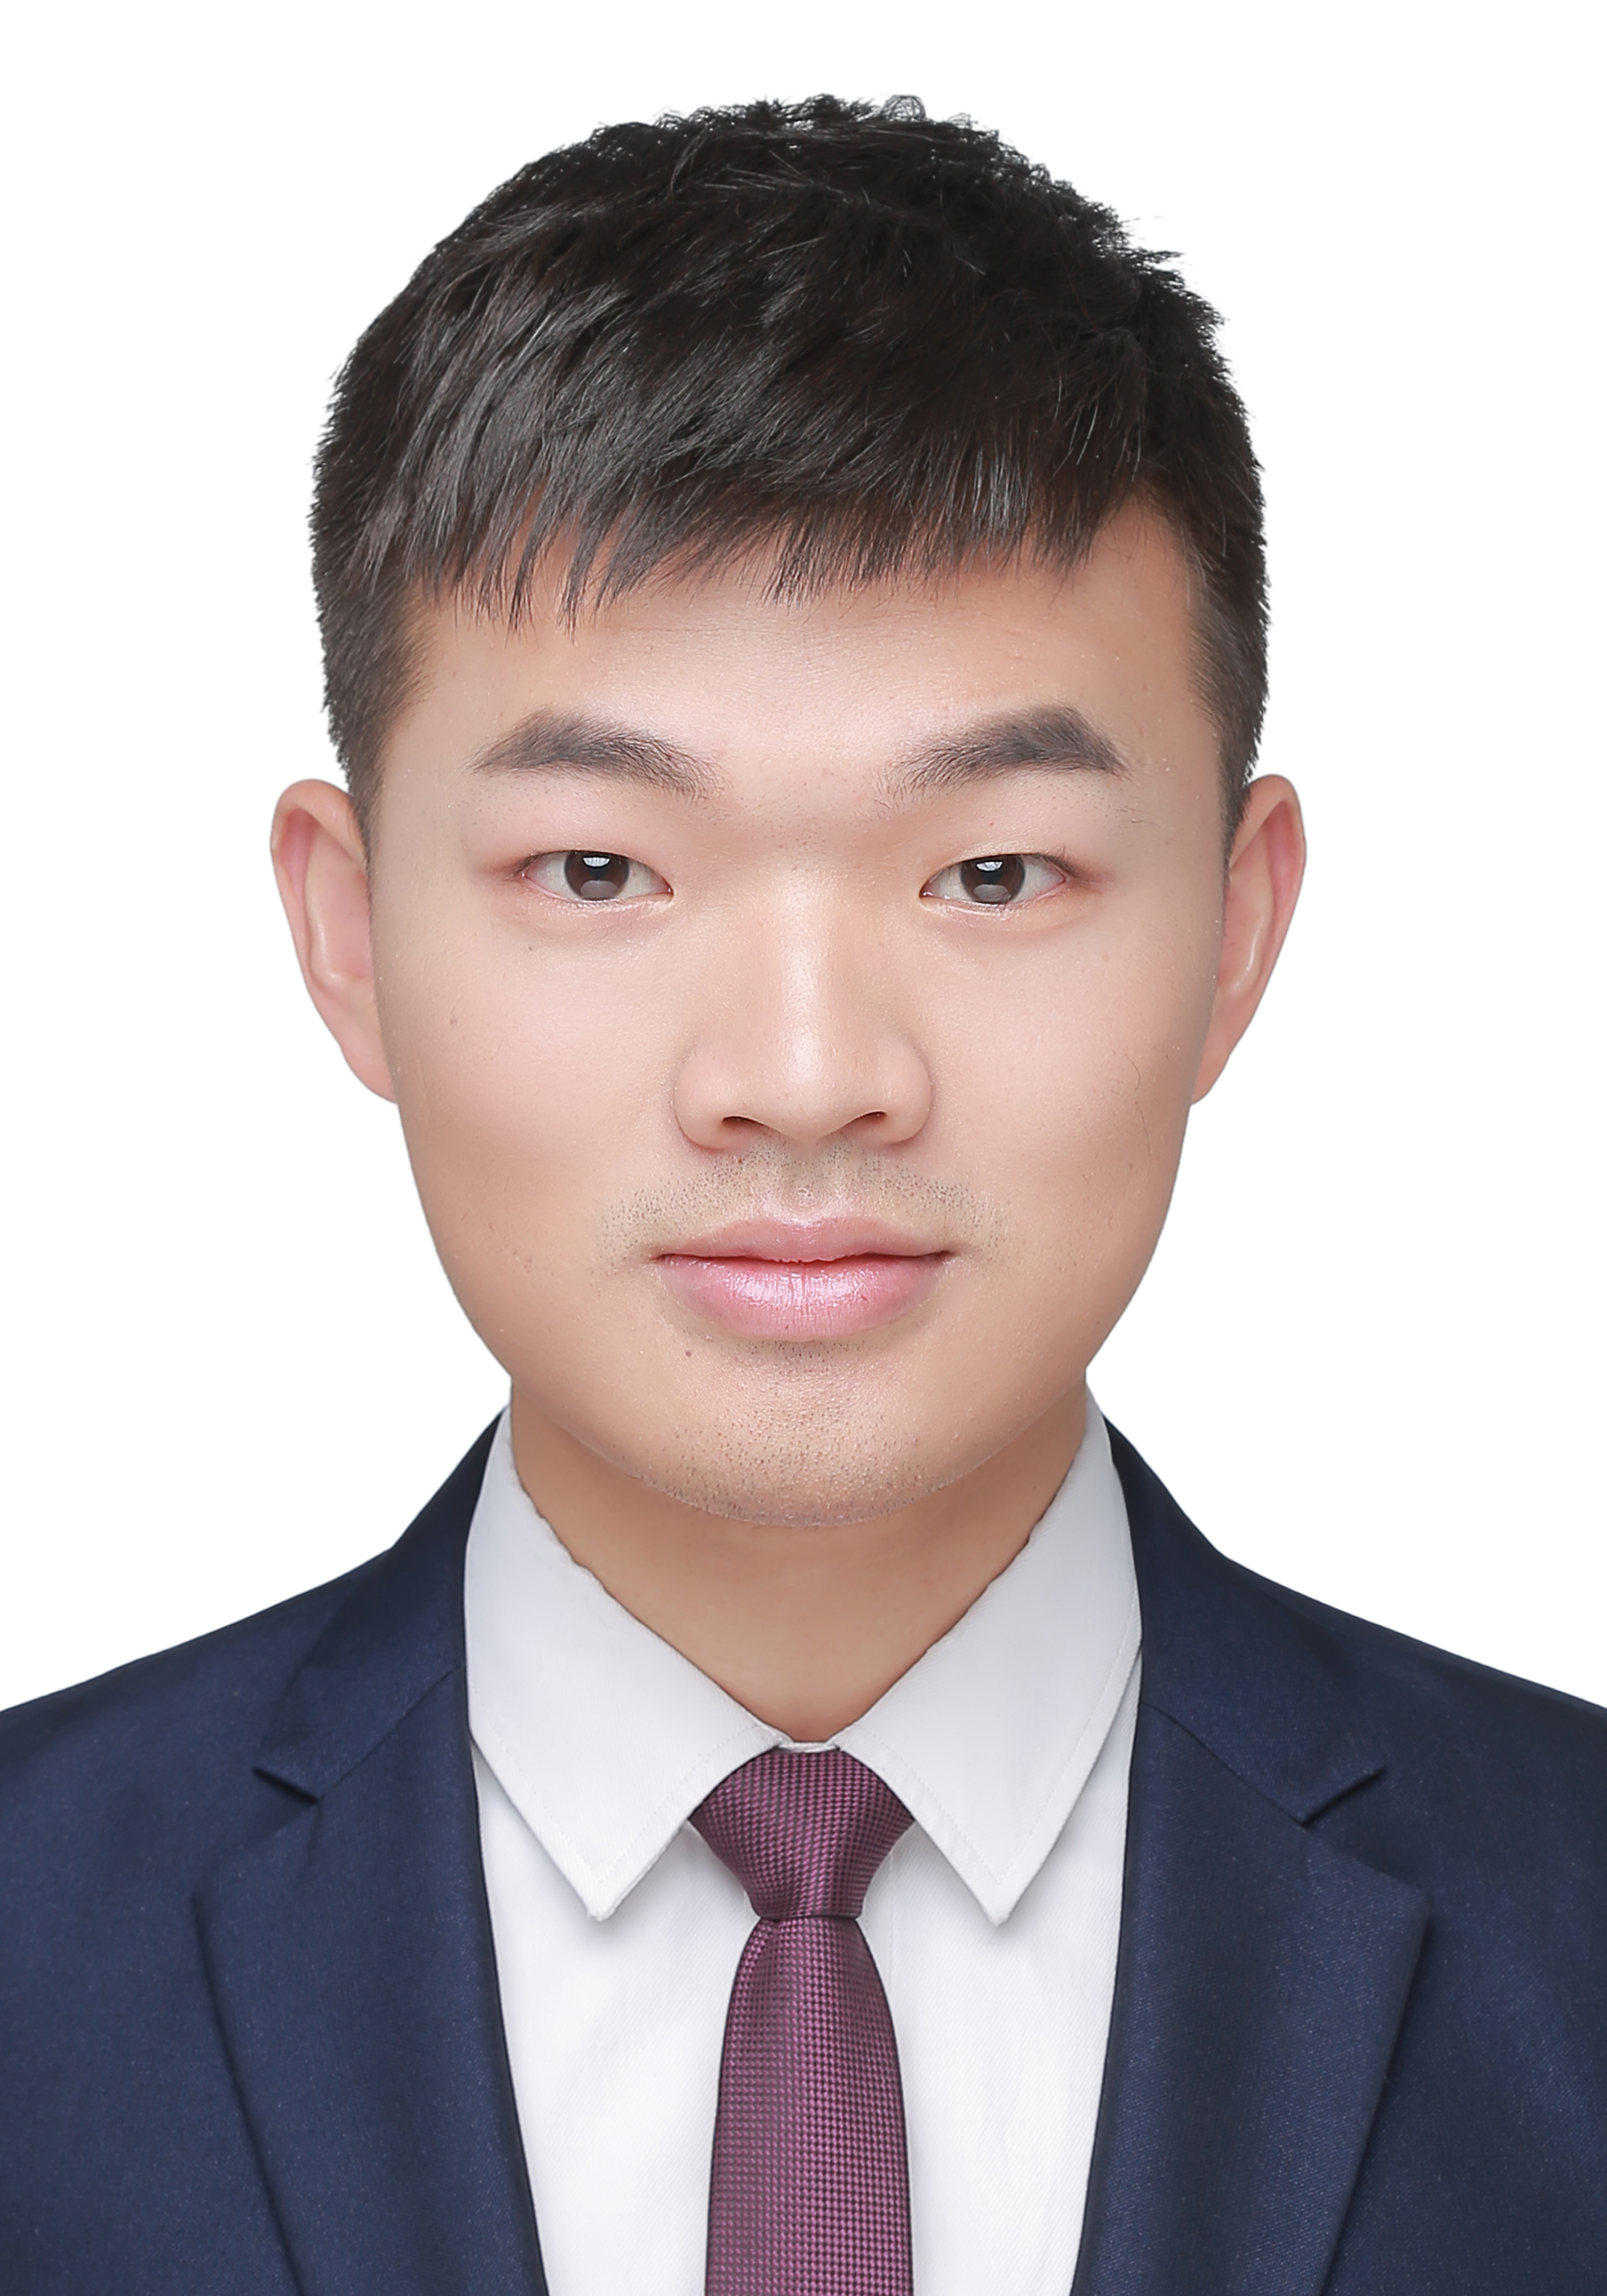
\includegraphics[width=0.88in]{avatar}
            }
        \end{tabu}
    }
    \columnbreak
    \Large{
        \begin{tabu}{ l l }
            & \faBirthdayCake{1995.09.12} \\
            & \phone{(+86)17600535912} \\
            & \email{izhouwl@163.com} \\
            & \homepage[\textbf{\color{red}{www.zhouweilin.cn}}]{https://zhouweilin.cn} \\
            & \github[github.com/Si3ver]{https://github.com/Si3ver} 
        \end{tabu}
    }
    \columnbreak
    \Large{
        \begin{tabu}{ r }
            \multirow{5}{3.5in}{
                \name{周伟林}
                \basicInfo{
                    \faSmileO{意向职位:web前端研发}
                }
            }
        \end{tabu}
    }
\end{multicols}

% 教育背景
\section{\faGraduationCap\  教育背景}
\datedsubsection{\textbf{北京邮电大学(211)\quad\quad\quad}{ 计算机科学技术\quad\quad\quad }{ 硕士 }}{2016年09月 -- 2019年06月}
\datedsubsection{\textbf{北京工业大学(211)\quad\quad\quad}{ 信息安全\quad\quad\quad\quad\quad\quad }{ 本科 }}{2012年09月 -- 2016年06月}

% 实习经历
\section{\faBriefcase\ 实习经历}
\datedsubsection{\textbf{滴滴出行\quad\quad\quad\quad\quad} \textbf{质量技术部\quad\quad\quad}{ WEB前端研发}}{2018年06月 -- 2018年09月}
\begin{itemize}
    \item[\faCheck] 参与月光宝盒(订单流量重放平台)和Omega(数据与产品质量检测管理平台)两个项目
    \item[\faCheck] 使用轻量级\textbf{\color{red}{模板引擎simplite}}开发用户反馈系统、启动崩溃分析系统的多个页面
    \item[\faCheck] 修改JSError和JSMonitor系统页面。增加表头冻结等feature,并重构代码
    \item[\faCheck] 使用\textbf{\color{red}{ECharts}}进行数据可视化,为页面添加柱状图、饼图和折线图,实现丰富的交互效果
    \item[\faCheck] 向后台索要接口数据格式,利用mock假数据,实现本地前后端分离开发
    \item[\faCheck] 页面国际化,使网站支持中英文一键切换
    \item[\faCheck] 成果:1. 页面上线到正式系统中,供公司内部使用 2. \textbf{\color{red}{重构代码}}后,减少了数据请求量
\end{itemize}

\datedsubsection{\textbf{西门子中国\quad\quad\quad\quad} \textbf{新闻传播部\quad\quad\quad}{网站技术支持}}{2017年10月 -- 2018年03月}
\begin{itemize}
  \item[\faCheck] 负责维护新的新闻发布平台AEM和旧平台SharePoint,以及旧系统到新系统的数据迁移
  \item[\faCheck] 为不同页面添加样式,如4列多栏的视频布局
  \item[\faCheck] 为asp页面开发公用组件,如Slider组件,利用iframe嵌入
  \item[\faCheck] 获取网站埋点数据的统计结果,整理每月PV/UV报表。
  \item[\faCheck] 收获:1. 邮件使用英文沟通,与老外口语交流,锻炼了英语听说读写 2. 接触到大型新闻发布系统的运维。
\end{itemize}

\datedsubsection{\textbf{北京江南天安科技\quad} \textbf{软件研发部\quad\quad\quad}{Windows程序开发}}{2015年07月 -- 2015年09月}
\begin{itemize}
  \item[\faCheck] 负责云密码机的专用UKey初始化工具和双因子认证软件的windows开发
  \item[\faCheck] 收获:1. 掌握了windows程序设计和VS的调试 2. 加深了对安全通信和密码学的理解。
\end{itemize}

% % 项目经历
% \section{\faUsers\ 项目经历}
% \datedsubsection{\textbf{H5移动端小游戏\quad\quad\quad}{别踩白块儿}}{2018年02月}
% \begin{onehalfspacing}
% \begin{itemize}
%   \item web版的别踩白块儿小游戏,实现自动加速、记录分数、调整难度等级等功能。
%   \item 使用canvas绘图,以MVC设计模式组织代码。采用响应式布局,并对移动端事件适配。白块儿移动有平滑的过渡效果。
%   \item 丰富了移动端的开发经验。
% \end{itemize}
% \end{onehalfspacing}
% \datedsubsection{\textbf{SVNF\quad\quad\quad\quad\quad\quad\quad\quad}{动态流量分配算法的设计与实现}}{2018年07月 -- 08月}
% \begin{onehalfspacing}
% \begin{itemize}
%   \item 经过调研发现,在VNFaaS部署到数据中心拓扑的过程中,VS(Vertical Scalability)、FPL(Flow Path Length)、SU(Server Utility)三者不能同时做到。
%   \item 本人提出并实现了SVNF和SVNF-adv启发式算法,借鉴了匈牙利算法的二分图最大匹配算法,最大化最小服务器可扩展性。
%   \item 与经典的CLBP方案相比较,通过最优化的预留资源方法,本方案能降低15\%~40\%丢包率,并且能保证较短的路由路径长度和较高的服务器利用率。
%   \item 锻炼了研究性思维,加深了对NFV、TE、启发式算法的理解。
% \end{itemize}
% \end{onehalfspacing}

% 技能树
\section{\faCogs\ 技能树}

\begin{itemize}
  \item[\faCheck] 熟悉原生JavaScript、ES6,有\textbf{\color{red}{H5移动端小游戏}}开发经验
  \item[\faCheck] 熟悉前后端分离、前端工程化,会配置Webpack,能使用Redux管理数据
  \item[\faCheck] 熟悉常用工具/库,包括\textbf{\color{red}{React.js}}、Canvas、ECharts、Bootstrap、AntD、jQuery、
  \item[\faCheck] 熟悉密码学、网络安全,理解\textbf{\color{red}{HTTPS}},有思科ASA防火墙配置经验和网络安全协议开发经验
  \item[\faCheck] 熟悉python可视化库Matplotlib、排版工具Markdown、LaTex
  \item[\faCheck] 通过CET-6,无障碍阅读英文文档,熟练使用Google、Stack Overflow检索
\end{itemize}


% 个人荣誉
\section{\faHeartO\ 论文与竞赛}

\trophy[Weilin Zhou, Yuan Yang, Mingwei Xu, “Accommodating dynamic traffic immediately: a VNF placement approach,” Orlando, USA, Nov. 2018.(IPCCC'18,SCI,CCF推荐会议,评审中)]{https://github.com/Si3ver/SVNF}

\trophy[周伟林, 杨芫, 徐明伟. 网络功能虚拟化技术研究综述. 计算机研究与发展, 2018, 55(4): 675-688. (国内计算机领域三大核心期刊之一,EI)]{http://crad.ict.ac.cn/CN/abstract/abstract3662.shtml}

\trophy[2015 思科网院杯(全国大学生网络竞赛) 本科组二等奖,全国排名第12]{http://www.catc.edu.cn/2015cup/news/19rr5gvqfnqk2.xhtml} 
\end{document}
